\chapter{Wstęp teoretyczny}



\section{Historia i stan obecny dziedziny}
Dynamiczny rozwój grafiki komputerowej obserwujemy od roku 1950 kiedy to w Massachusets Institute of Technology \cite{jankowski} powstał pierwszy
komputer wyposażony w grafoskop. Obecnie większość użytkowników nie potrafi sobie wyobrazić komputera bez graficznego interfejsu.
Coraz większe możliwości nowoczesnych komputerów są motorem napędowym rozmaitych badań nad komputerowymi modelami świata rzeczywistego.

Prekursorem w dziedzinie wizualizacji drzew był polski matematyk Stanisław Ulam, przedstawiajac w 1962r. \cite{ulam} drzewo jako samoorganizującą się
strukturę. Jego model wykorzystujący automaty komórkowe opierał się na rywalizacji węzłów  drzewa o przestreń.
Honda zaproponował w 1971r. modelowanie drzew jako stuktury rekursywnej opisanej
zbiorem parametrów takich jak kąt rozgałęzień, czy stosunek długości między kolejnymi poziomami rekurencji \cite{honda}.

Dopiero w latach osiemdziesiatych
możliwości uwczesnych komputerów pozwoliły na trójwymiarową wizualizację drzew, czego przykładem może być praca Bloomenthala z 1985r. \cite{bloomenthal}
przedstawiająca proces modelowania klonu. Podejście do tematu możemy podzielić na dwie grupy:
\begin{itemize}
\item od ogółu do szczegółu, czyli modelowanie z zadanymi parametrami wyglądu drzewa
\item od szczegółu do ogółu, czyli opisanie pewnym zbiorem parametrów budowy drzewa
\end{itemize}
Problem stworzenia modelu drzewa możemy podzielić na stworzenie modeli jego składowych np. gałęzi, kory, liści, czy kwiatów i późniejsze
ich połączenie w jedną całość. Na chwilę obecną istnieją zaawansowane metody generowania zarówno całych drzew, jak i poszczególnych jego części.

\section{Generowanie drzewa}
Generowanie drzewa przebiega w następujących etapach:
\begin{itemize}
\item generowanie szkieletu
\item stworzenie geometrii
\item teksturowanie
\item edycja
\end{itemize}
\begin{center}
	\includegraphics[width=120mm]{images/colonization/generation.png}
	\captionof{figure}{Etapy tworzenia modelu drzewa \cite{spaceColonization}}
	\label{colonization_generation}
\end{center}
\subsection{Algorytm kolonizacyjny}
Algorytm kolonizacji przestrzeni dalej nazywany algorytmem kolonizacyjnym opiera się na biologicznym aspekcie rywalizacji roślin o dostępną wokół nich przestrzeń. 
Po raz pierwszy został zaprezentowany w 2007 roku \cite{spaceColonization}, będąc rozszerzeniem na przestrzeń trójwymiarową metody generowania liści przy wykorzystaniu systemów cząsteczkowych \cite{particleMethod}. 
Podstawową ich ideą było umieszczanie cząstek w obrysie liścia, a następnie śledzenie ich ruchu w kierunku szypułki uwzględniając wzajemne przyciąganie cząstek. 
Z biologicznego punktu widzenia miało to uzasadnienie jako śledzenie trasy transportu substancji niezbędnych do życia rośliny. 
W podejściu kolonizacyjnym symuluje się iteracyjny wzrost gałęzi drzewa, aż do wykorzystania całego dostępnego miejsca.

\newpage
Pojęcia:
\begin{description}
	\item[węzeł drzewa] odcinek w przestrzeni trójwymiarowej reprezentujący część gałęzi
	\item[atraktor] punkt w przestrzeni trójwymiarowej, do którego osiągniecia dążą węzły drzewa
	\item[korona] podzbiór punktów przestrzeni trójwymiarowej
\end{description}
\subsection{Opis skrócony}
\begin{center}
	\includegraphics[width=120mm]{images/colonization/colonization.png}
	\captionof{figure}{Etapy algorytmu kolonizacyjnego \cite{spaceColonization}}
	\label{colonization_colonization}
\end{center}


\subsection{Algorytm}

Dane algorytmu:
\begin{my_itemize}
	\item{korona}
	\item{di - influence distance}
	\item{dk - kill distance}
	\item{D - node length}
	\item{points - liczba atraktorów}
	\item{dist(a,b) - funkcja zwracająca odległość euklidesową między dwoma punktami przestrzeni}
\end{my_itemize}

\begin{verbatim}
  rozmieść atraktory wewnątrz korony drzewa
  dodaj do drzewa węzeł główny
  dopóki istnieją atraktory:
    dla kazdego atraktora a :
      wyznacz najbliższy węzeł drzewa n
       jesli dist(n,a) <=di
        oblicz wektor n->a
      dodaj nowy wezel do drzewa (n-a)
  dla kazdego atraktora
    jeśli istnieje wezeł drzewa w odległosci <=dk
      usuń atraktor
\end{verbatim}

Ponieważ istnieją parametry uniemożliwiające zakończenie algorytmu np. $dk \ll D$, warunek końca obliczeń na potrzeby implementacji został zastąpiony sprawdzeniem, czy w poprzedniej iteracji utworzono jakiś nowy węzeł drzewa.

\section{Tworzenie geometrii modelu}
\subsection{Wstęp}
Rośliny, w szczególności drzewa, są bardzo złożonymi strukturami. Projektując model drzewa trzeba zwrócić uwagę na wiele aspektów takich jak: sposób łączenia gałęzi, przyrost grubości gałęzi, rozłożenie liści na drzewie, położenie pojedynczego liścia w przestrzeni, sposób przyłączenie liścia do gałęzi.


\subsection{Model węzła}
Węzeł charakteryzuje się dwoma parametrami: położeniem(P) oraz promieniem(R). Na ich podstawie wyliczany jest segment, który składa się z przynajmniej 3 punktów leżących na okręgu o środku w punkcie P i promieniu R. Wektor normalny do płaszczyzny tworzonej przez punkty segmentu oraz punkt P jest wyliczany w następujący sposób: $\vec{n}=\frac{\vec{AP}}{|\vec{AP}|}+\frac{\vec{PB}}{|\vec{PB}|}$, gdzie A - poprzednik P; B - następnik P. Jeśli węzeł A lub B nie istnieje, to odpowiednio pierwszy lub drugi składnik sumy przyjmuje wartość 0.

Promień danego węzła jest wyznaczany w nastepujący sposób:
$$
  R[node] = \left\{ 
  \begin{array}{l l}
    0.1 & \textrm{jeśli $size[node.children] == 0$}\\
    m*\sqrt[rf]{\sum_{i} R[node.children(i)]^{rf}}+a & \textrm{jeśli $size[node.children] > 0$}\\
  \end{array} \right.
$$
Oznaczenia:
\begin{description}
	\item[node] struktura otrzymana z algorytmu kolonizacyjnego;
	\item[node.children] lista węzłów potomnych;
	\item[\textrm{R[node]}] promień gałęzi w $node$;
	\item[\textrm{size[node.children]}] liczba elementów w liście $node.children$;
	\item[rf, m, a] współczynniki wpływające na grubość gałęzi (domyślne wartości: $rf=1.8$, $m=1$, $a=0$)
\end{description}

\begin{center}
	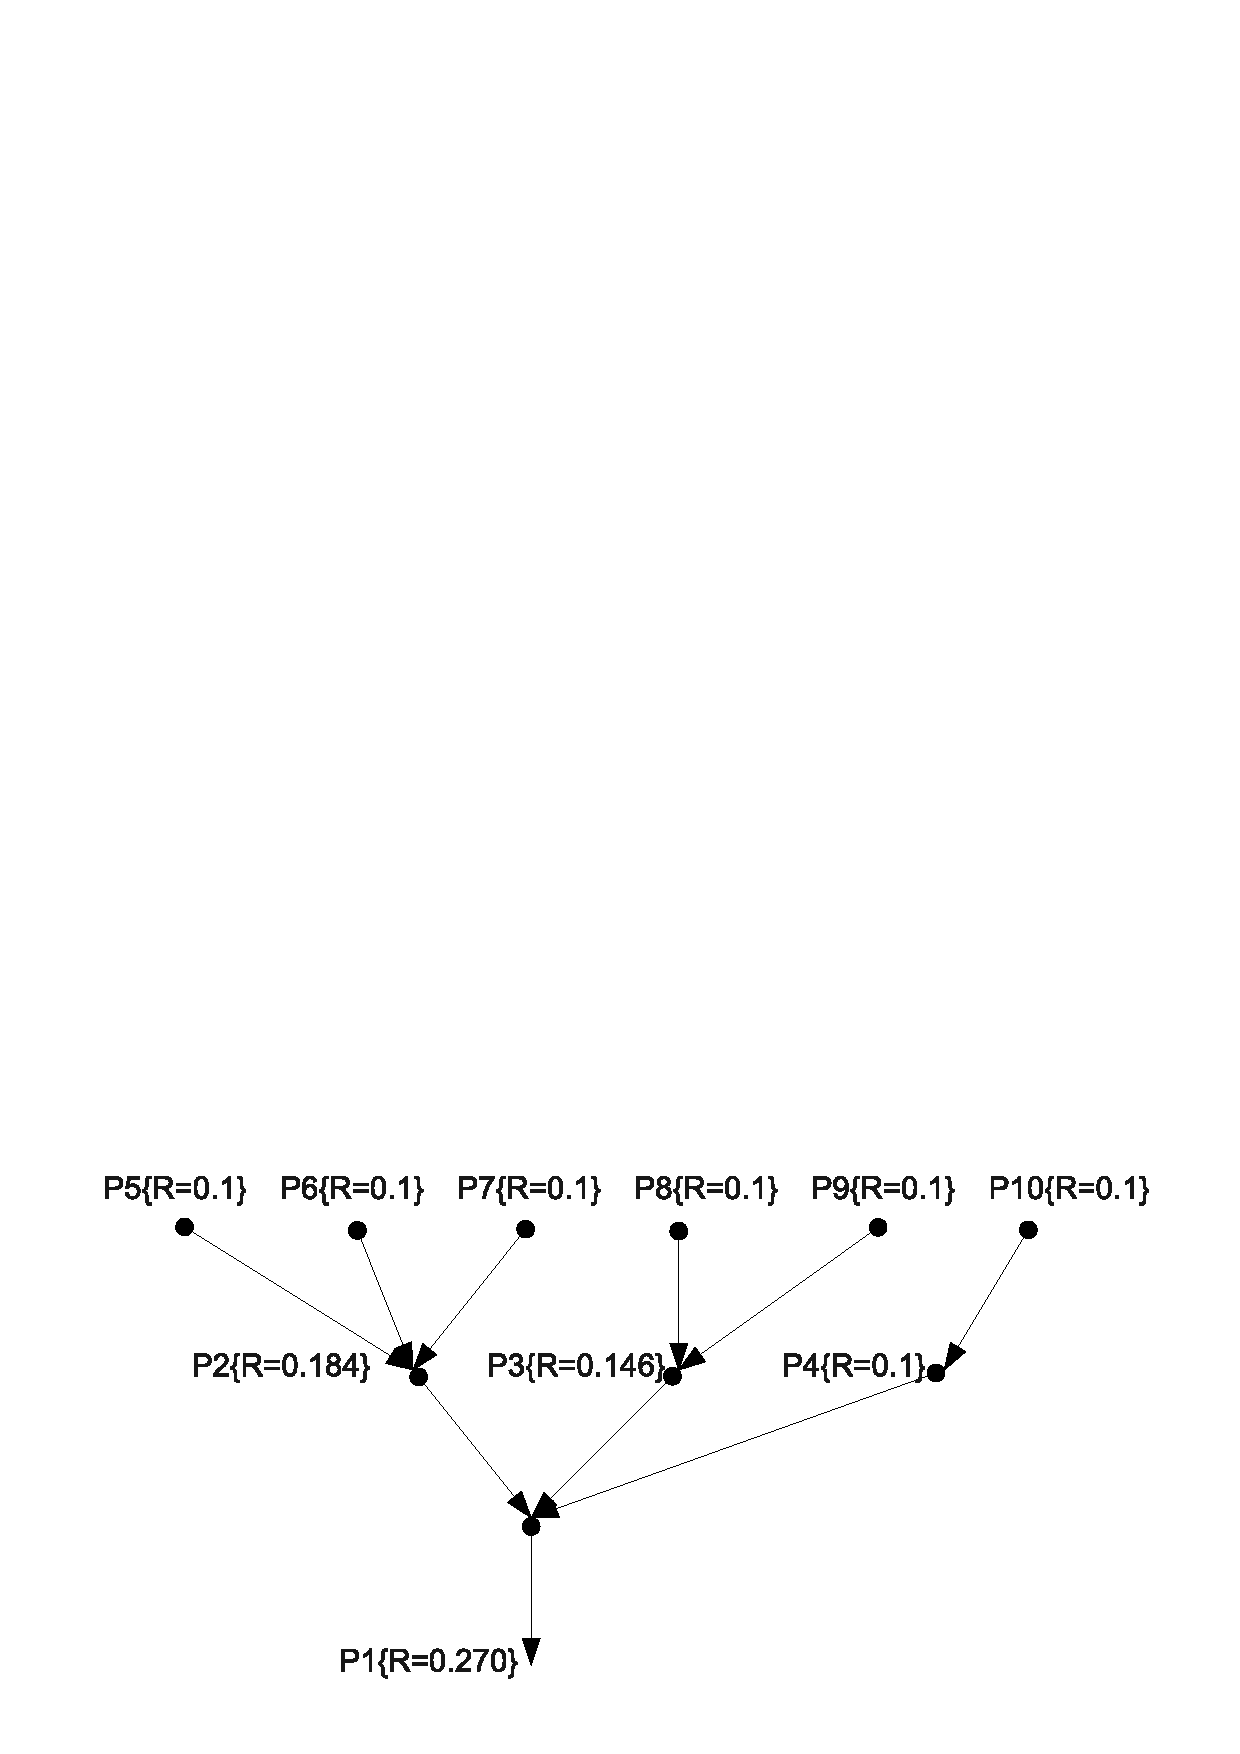
\includegraphics[width=130mm]{images/model/node_radius.pdf}
	\captionof{figure}{Obliczone promienie węzłów dla przykładowego drzewa.}
	\label{node_radius}
\end{center}


\begin{center}
	\includegraphics[width=130mm]{images/model/two_segments.png}
	\captionof{figure}{Dwa wyrenderowane segmenty wokół węzłów P1 i P2}
	\label{two_segments}
\end{center}

\subsection{Model gałęzi}
Dobrym przybliżeniem gałęzi jest uogólniony walec (ang. generalized cylinder). Jest to powierzchnia w przestrzeni $R^3$, której przekrój poprzeczny jest krzywą zamkniętą.

Gałąź jest reprezentowana przez listę kolejnych węzłów o największych średnicach idąc od dołu drzewa. Pozostałe węzły są początkami gałęzi potomnych. Przez połączenie ze sobą odpowiednich punktów z segmentów sąsiednich węzłów otrzymujemy uogólniony walec (rys. \ref{two_segments}).

Gałąź może być początkiem kolejnych konarów, dlatego posiada kolekcję gałęzi potomnych.

\begin{center}
	\includegraphics[width=130mm]{images/model/branching.png}
	\captionof{figure}{Fragment drzewa. Gałąź główna(kolor brązowy) w widocznym obszarze posiada 3 gałęzie potomne(kolor zielony).}
	\label{branching}
\end{center}
\subsection{Model liścia}
Liść cechuje się dwiema właściwościami: normalną do powierzchnii liścia oraz wektorem wyznaczającym kierunek liścia. Oba wektory są do siebie prostopadłe. Liść jest związany z konkretnym węzłem.

\begin{center}
	\includegraphics[width=80mm]{images/model/leaf_vects.png}
	\captionof{figure}{Liść z zaznaczonymi wektorami normalnym(zielony) i kierunkowym(czerwony). }
	\label{leaf_vect}
\end{center}

Wektor normalny jest wyznaczany na podstawie położenia liścia względem punktu (0,0,0). Dodatkowo jest obciążany wektorem grawitacji, którego współrzędna Z jest losowa z zakresu $\langle-0.9;0\rangle$. 



Liście są rozkładane są na gałęziach w sposób losowy, przy czym rozkład nie jest równomierny. Prawdopodobieństwo umiejscowienia liścia na końcu gałęzi jest znacznie większe niż na początku. Efekt ten uzyskaliśmy w następujący sposób: $node\_id = \lceil\sqrt{rand()}*(nodes\_length-1)\rceil$.

\begin{description}
	\item[node\_id] indeks węzła w danej gałęzi, do którego zostanie doczepiony liść
	\item[nodes\_length] jest liczbą węzłów należących do danej gałęzi.
	\item[rand()] zmienna losowa o rozkładzie równomiernym z zakresu $(0;1\rangle$
\end{description}

\subsection{Wygładzanie gałęzi przy pomocy algorytmu Chaikina \cite{smoothing}}
\subsubsection{Wstęp}
W 1974r. George Chaikin opublikował algorytm generowania krzywych ze skończonej liczby punktów kontrolnych. Algorytm ten okazał się bardzo interesujący przez niski stopień swojej komplikacji. Opiera się jedynie na ścinaniu wierzchołków początkowego wielokąta.

Tworzenie krzywej następuje iteracyjnie. Proces można można powtarzać, aż do osiągnięcia wymaganej rozdzielczości krzywej (rys. \ref{chaikin_1}).

\begin{center}
	\includegraphics[width=80mm]{images/model/chaikin_1.png}
	\captionof{figure}{Kolejne iteracje algorytmu Chaikina. \cite{smoothing}}
	\label{chaikin_1}
\end{center}

\subsubsection{Opis algorytmu}

Dla danego wielokąta \{$P_1$, $P_2$, ..., $P_n$\} wyznaczamy wielokąt pochodny \{$R_1$, $L_1$, $R_2$, $L_2$, ..., $R_n$, $L_n$\}, gdzie
$L_i = \frac{1}{4}P_{i-1} + \frac{3}{4}P_i$ oraz $R_i = \frac{3}{4}P_i + \frac{1}{4}P_{i+1}$.
Nowo powstały wielokąt składa się z $2n$ wierzchołków.

\begin{center}
	\begin{picture}(200,100)
		\put(10,10){\circle*{5}}
		\put(5,15){$P_{i-1}$}
	
		\put(90,70){\circle*{5}}
		\put(85,75){$P_i$}
	
		\put(190,20){\circle*{5}}
		\put(175,25){$P_{i+1}$}
	
		\put(10,10){\line(4,3){80}}
		\put(90,70){\line(2,-1){100}}
		
		\put(70,55){\circle*{5}}
		\put(65,60){$L_i$}
		\put(115,57.5){\circle*{5}}
		\put(110,62.5){$R_i$}
		
		\multiput(70,55)(10,0){5}{\line(1,0){5}}
		
	\end{picture}
	\captionof{figure}{Wierzchołki pochodne dla $P_i$.}
\end{center}

\subsubsection{Zastosowanie algorytmu Chaikina dla gałęzi}
Algorytm Chaikina w podstawowej wersji dla każdego punktu do wyznaczenia wierzchołków pochodnych, wymaga 2 sąsiadów. Chcąc zastosować wcześniej wspomnianą metodę dla gałęzi (łamana otwarta), trzeba wprowadzić pewne modyfikacje podczas przekształcania jej końców.


\begin{itemize}
	\item{Dla $i=1$ lub $i=n$: $L_i = R_i = P_i$}
	\item{Dla $i=2$: $L_i = \frac{1}{2}P_{i-1} + \frac{1}{2}P_i$ oraz $R_i = \frac{3}{4}P_i + \frac{1}{4}P_{i+1}$}
	\item{Dla $i=n-1$: $L_i = \frac{1}{4}P_{i-1} + \frac{3}{4}P_i$ oraz $R_i = \frac{1}{2}P_i + \frac{1}{2}P_{i+1}$}
	\item{Dla pozostałych przypadków: $L_i = \frac{1}{4}P_{i-1} + \frac{3}{4}P_i$ oraz $R_i = \frac{3}{4}P_i + \frac{1}{4}P_{i+1}$}
\end{itemize}

\begin{center}
	\includegraphics[width=130mm]{images/model/chaikin_branch.pdf}
	\captionof{figure}{Kolejne iteracje algorytmu Chaikina dla łamanej otwartej.}
	\label{chaikin_branch}
\end{center}

\subsection{Korona - TODO}
Algorytm kolonizacyjny w pierwszym kroku rozmieszcza atraktory wewnątrz danej podprzestrzenii, która to determinuje swoim kształtem wygląd wygenerowango drzewa. Wybór typu korony został ograniczony do 3 kształtów.
\begin{itemize}
	\item{sfera - możliwość zmiany promienia}
	\item{ścięty stożek - możliwość zmiany wysokości oraz promiania dolnej i górnej podstawy}
	\item{\textit{spline crown} - korona tworzona na skutek obrotu krzywej sklejalnej trzeciego stopnia wokół osi OX}
\end{itemize}

\begin{center}
	\includegraphics[width=130mm]{images/model/crowns.png}
	\captionof{figure}{Typy koron (sfera, ścięty stożek, \textit{spline crown})}
	\label{crowns}
\end{center}

\section{Teksturowanie}
Aplikacja obsługuje jedynie tekstury w formacie 24bit BMP. 
Ponadto wymiary tekstur w pikselach muszą być potęgą dwójki.
Dla tekstur liści aplikacja interpretuje kolor czarny jako ${100\%}$ przeźroczystość tekstury.

Ułożenie tekstury kory na pniu można regulować za pomocą parametrów:
\begin{itemize}
\item ${kx}$ -liczba tekstur potrzebna do owinięcia pnia
\item ${ky}$ - stosunek rozmiaru tekstury do odległości mierzonej wzdłuż pnia
\end{itemize}
Poniżej przedstawiono przykładowy fragment pnia drzewa utworzony dla ${kx=2}$ i ${ky=(0.2..0.5)}$
\begin{center}
	\includegraphics[width=140mm]{images/textures/ky.png}
	\captionof{figure}{Wpływ współczynnika ky na wygląd pnia. }
	\label{ky_texture}
\end{center}
Poniżej przedstawiono przykładowy fragment pnia drzewa utworzony dla ${ky=0.5}$ i ${kx=(1..4)}$
\begin{center}
	\includegraphics[width=140mm]{images/textures/kx.png}
	\captionof{figure}{Wpływ współczynnika kx na wygląd pnia. }
	\label{kx_texture}
\end{center}

